
%TODO: 64-bit core?

The ISE designs were integrated with the \CORE{2} core as a base platform
for evaluation.
The \CORE{2}\footnote{%
  \ifbool{anonymous}{Details of this core have been anonymised to comply with the TCHES submission guidelines.}{}
} core
implements the {\tt rv32imc} instruction set: 32-bit base ISA, with the
Multiply and Compressed instruction set extensions.
A block diagram of the core is shown in~\REFFIG{fig:design:cpu_block:2}.
A standard 5-stage, in-order pipeline is used, which
means that each stage of execution
(namely fetch, decode, execute, memory access, and write-back)
occurs in {\em parallel} for multiple different in-flight instructions.

Note there are two memory interfaces, one for (instruction) fetch and one for
(data) memory accesses;
no form of cache hierarchy or branch prediction is implemented.
The core implements various performance counters,
and
elements of the
RISC-V Privileged Resource Architecture (PRA)~\cite[Chapter 3]{RV:ISA:II:17}
related to exception and interrupt handling.

To support the AES ISE variants, two modifications were made to the core:
1) The Instruction Decode module was modifed to support identification and
   operand selection for the new instructions. 
2) A new ``AES" functional unit (AES FU) was added in the execute stage to
   perform the instruction computations.
Because all of the variants read at most two,
and write one general purpose register, no new structural datapaths
were needed.

All of the AES variants share the same sets of inputs, so the interface
to the AES FU is kept constant for every variant.
A synthesis time parameter was then added to switch between different
ISE variants.
The following sections describe each ISE variant using pseudo-code, and
give a simplified datapath diagram for the AES FU internals.

\begin{figure}
\centering
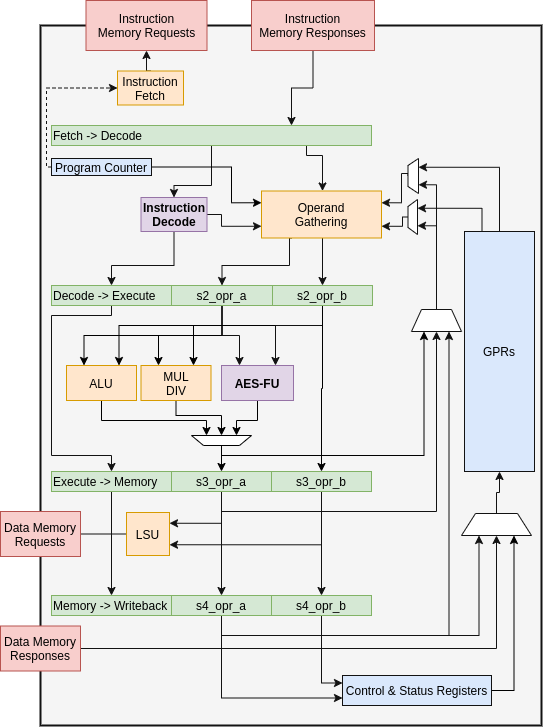
\includegraphics[scale=0.5,angle=90]{diagrams/scarv-cpu-uarch.png}
\subcaption{Core $2$: \CORE{2}.}
\label{fig:design:cpu_block:2}
\end{figure}

% TODO move or split into pieces.
\begin{figure}
\centering
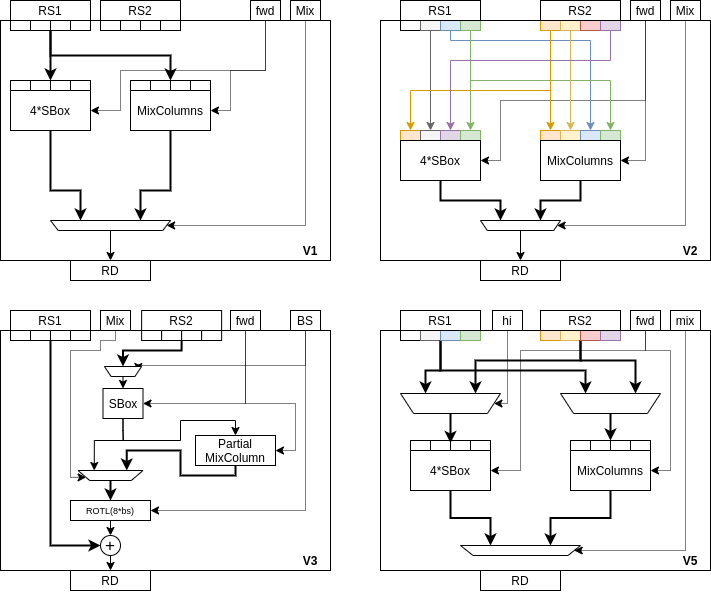
\includegraphics[scale=0.5]{diagrams/ise-datapaths.png}
\subcaption{Datapath diagrams for the four 32-bit ISE variants.}
\label{fig:design:fu_block:2}
\end{figure}
